%%%%
%% Design :: User Interface
%%%
\section{User Interface}
\label{sec:design_user_interface}

The previous sections have presented a number of system designs from a 
programmatic point of view. Within this section, there will be a focus upon 
user interface designs, and thus how the end user will interact with the system.

Fundamentally there are two aspects to the user interface design of the system 
--- inputting the clue and retrieving the results. Each of these aspects will 
be discussed in more detail in the following subsections.


%%%
%% Design :: User Interface :: Platform Support
%%%
\subsection{Platform Support} 
\label{sub:platform_support}

One of the main objectives of the project is to develop a system that can be 
used upon a number of mobile platforms, as well as trying not to neglect 
`traditional' desktop users.

In order to complete both of these objectives, a responsive design is required.
A responsive design is one that is able to dynamically change based upon the 
screen size.

This means that there will only be one code based for multiple screen sizes, and
thus allows for easier maintainability. All of the designs within this section 
feature a responsive design. Figure \ref{fig:input_form_compare} illustrates the
power of responsive designs.

The left-hand side form shows a `traditional' desktop experience, whilst the 
form upon the right-hand side, shows a mobile experience.

\begin{figure}[H]
  \centering
  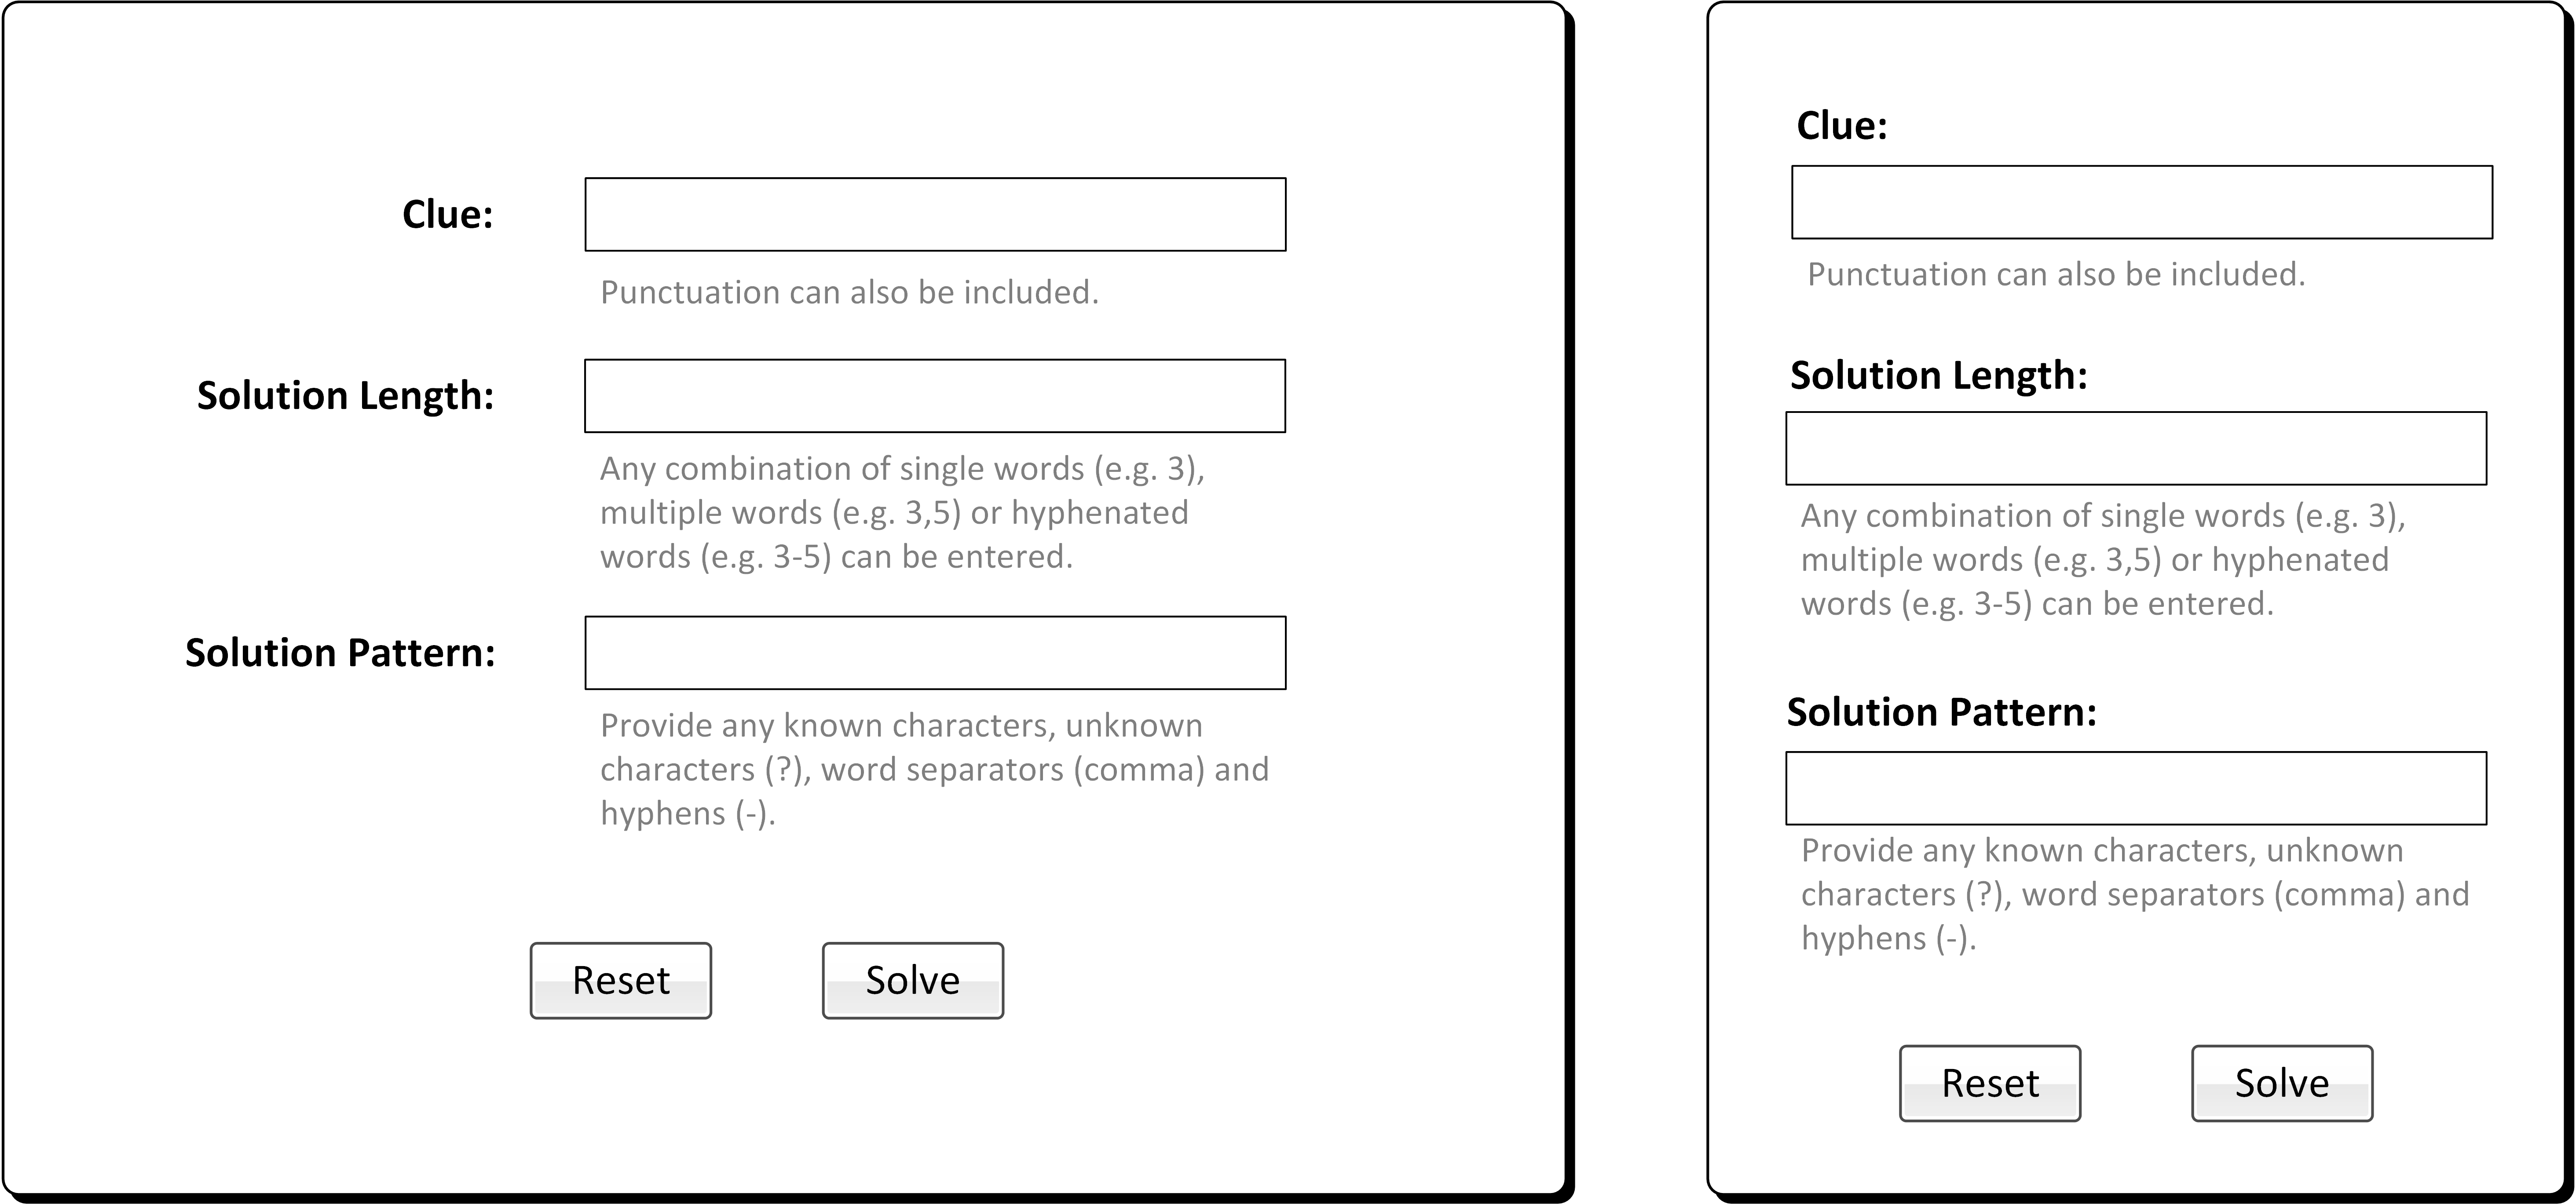
\includegraphics[width=0.8\textwidth]{ui/form_comparison.jpg}
  \caption{The input form to be completed by the end user}
  \label{fig:input_form_compare}
\end{figure}


%%%
%%  Design :: User Interface :: User Input
%%%
\subsection{User Input} 
\label{sub:user_input}

In order for the system to solve the clue, it must first be given the clue, 
along with additional supporting information. The additional information such as 
the solution length and solution pattern is vital to the system in order for it 
to compute the correct answer. 

However the intended users of the system are likely to be operating upon some 
form of mobile device, meaning that a simple and power interface is required. It
also means that space will be at a premium, and thus it can not afford to be 
wasted.

Figure \ref{fig:input_form} illustrates the design of the user input form. One 
of the most noticeable elements to the form design is how much space has been 
allocated to the input boxes. 

The design of the inputs utilises a bi-column setup using the ratio of 1:3. This
means that for every 1 pixel of space allocated to the left-hand labels, there 
will be 3 pixels of space allocated to the right-hand input boxes. This allows 
users of mobile devices to quickly select the input box, rather than having to 
tap a small area several times.

In order to assist the end user additional help blocks will be included, and 
give useful information to the user, such as describing the solution pattern 
format required.

\begin{figure}[H]
  \centering
  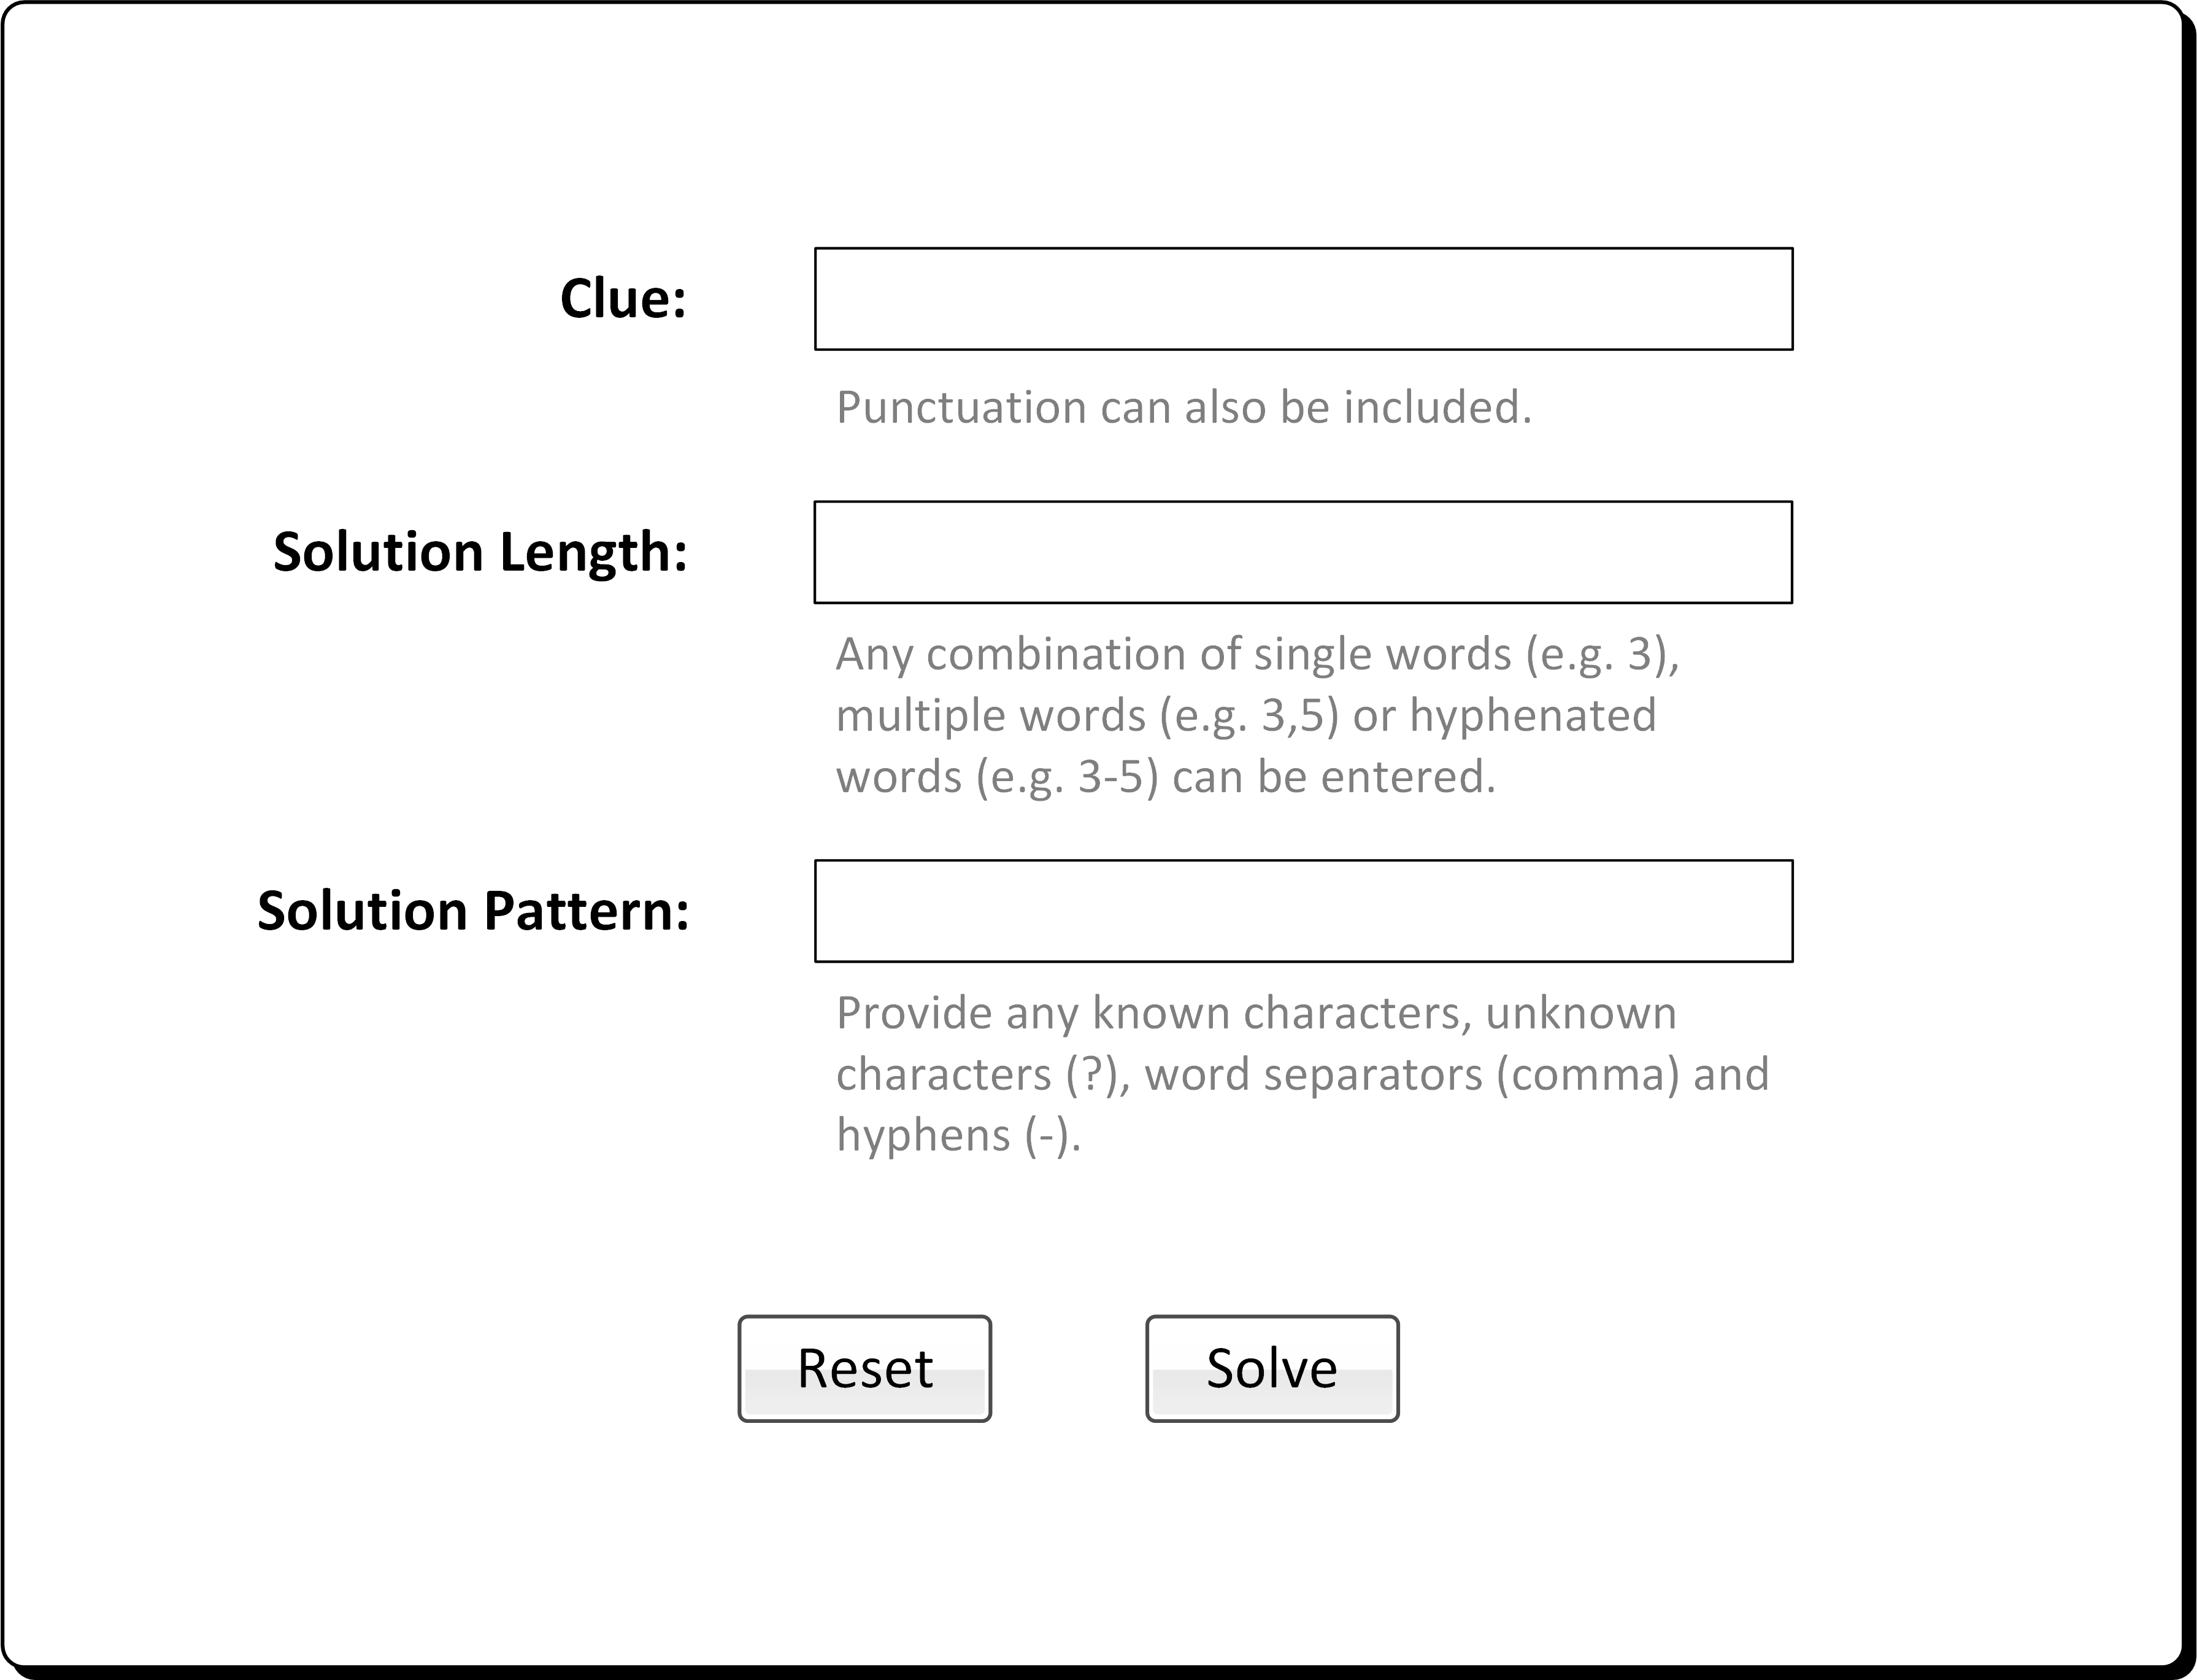
\includegraphics[width=0.8\textwidth]{ui/form.jpg}
  \caption{The input form to be completed by the end user}
  \label{fig:input_form}
\end{figure}

As the system is dealing with input from users, it is inevitable that a user 
will attempt to input incorrect data. This will require validation to be 
performed, and if validation has failed then the user should be notified. 

As previously mentioned space is a premium upon a mobile device. Therefore 
displaying a list of validation error messages at the top of the screen would 
not be utilising limited amount of space wisely.

In order to combat this issue, validation will be displayed `inline' with the 
form input elements, as seen within figure \ref{fig:input_form_error}. By 
utilising an `inline' approach it recycles the screen space that has been made 
available to the form.

For inputs that have passed the validations the outline will change to green, 
and for validations that have failed the input group will change to red. This 
will immediately alert the user to the various issues, and thus allows the user 
to fix the errors in a quicker and more efficient manner.

\begin{figure}[H]
  \centering
  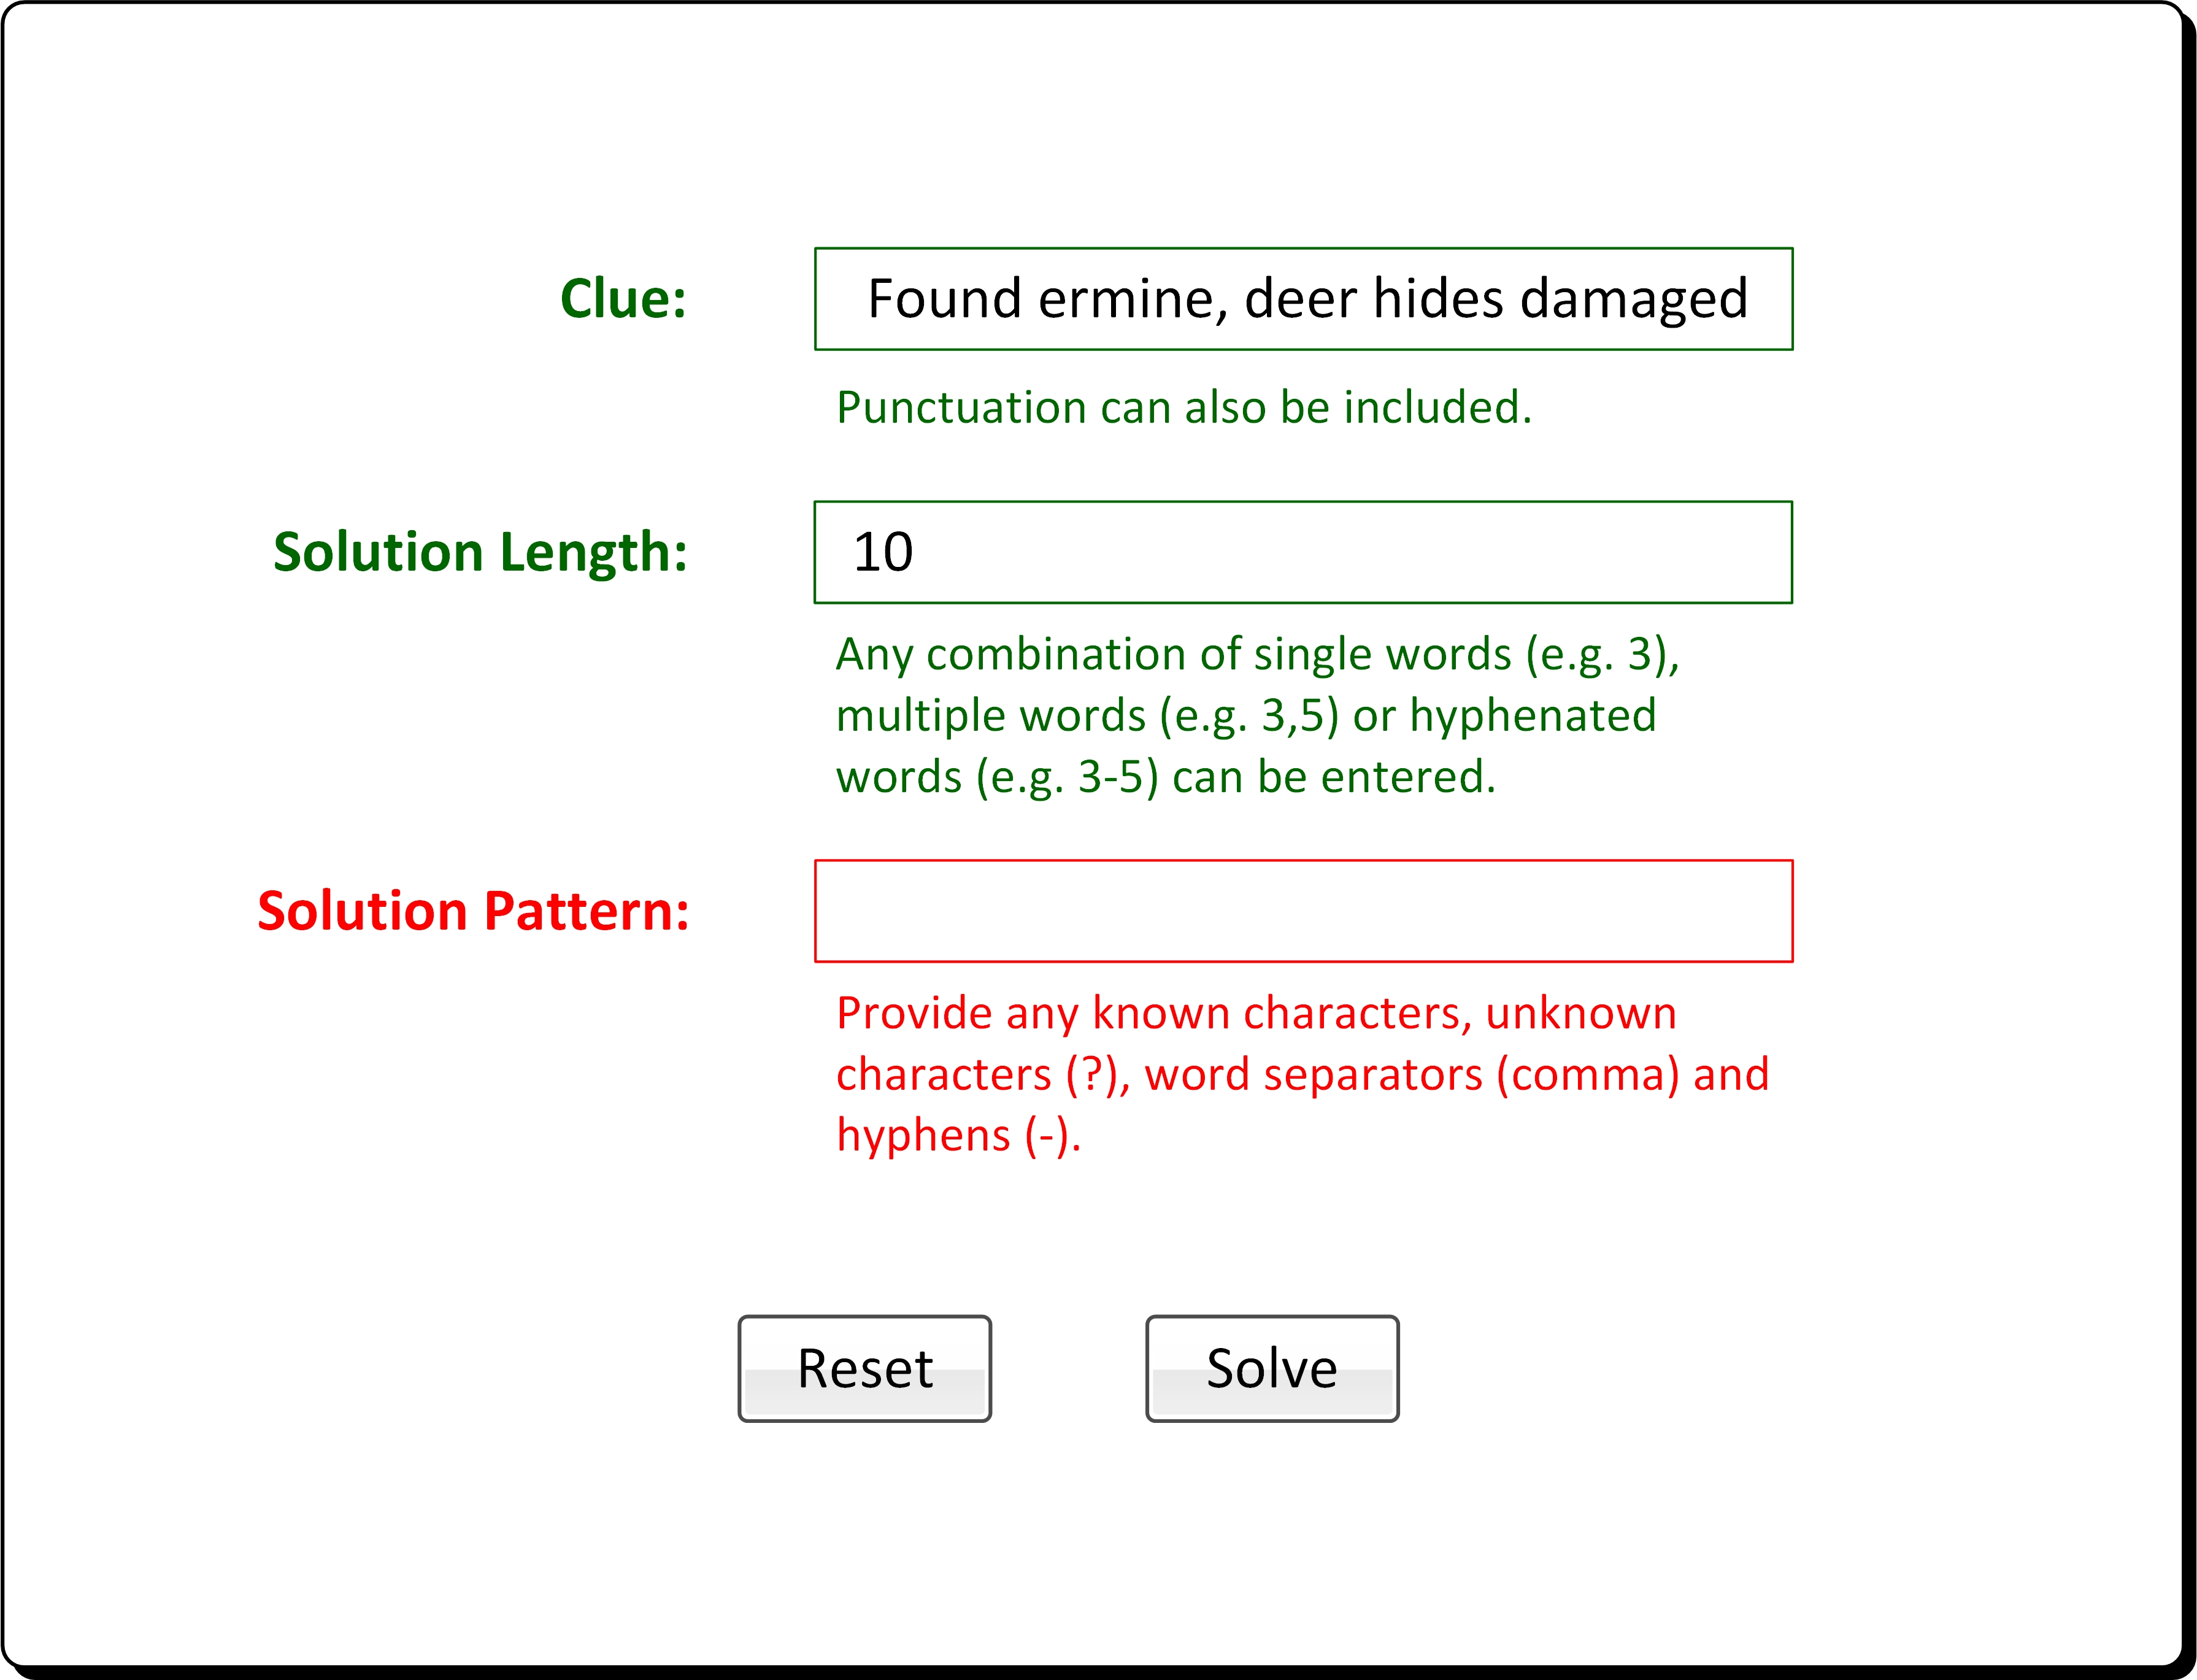
\includegraphics[width=0.8\textwidth]{ui/form_error.jpg}
  \caption{The input form indicating a validation error}
  \label{fig:input_form_error}
\end{figure}


%%%
%% Design :: User Interface :: Results
%%%
\subsection{Results} 
\label{sub:results}

The displaying of the results follows on from some of the previous design 
decisions. Each potential solution is rendered into it's own panel, and will 
contain the confidence rating, and the solver type that managed to deduce the 
solution (as shown in Figure \ref{fig:results_primary}).

Within an open panel, additional information is displayed --- known as the 
solution trace. A solution trace provides a step by step account of how the 
solution was able to be computed. The solution trace may help to teach users how
a particular type of clue is solved.

The results are ordered by confidence rating in ascending order, and by default 
the first panel will be `open', showing the solution trace. The reason for this
is that the top answer is likely to be the answer the end user is looking for

\begin{figure}[H]
  \centering
  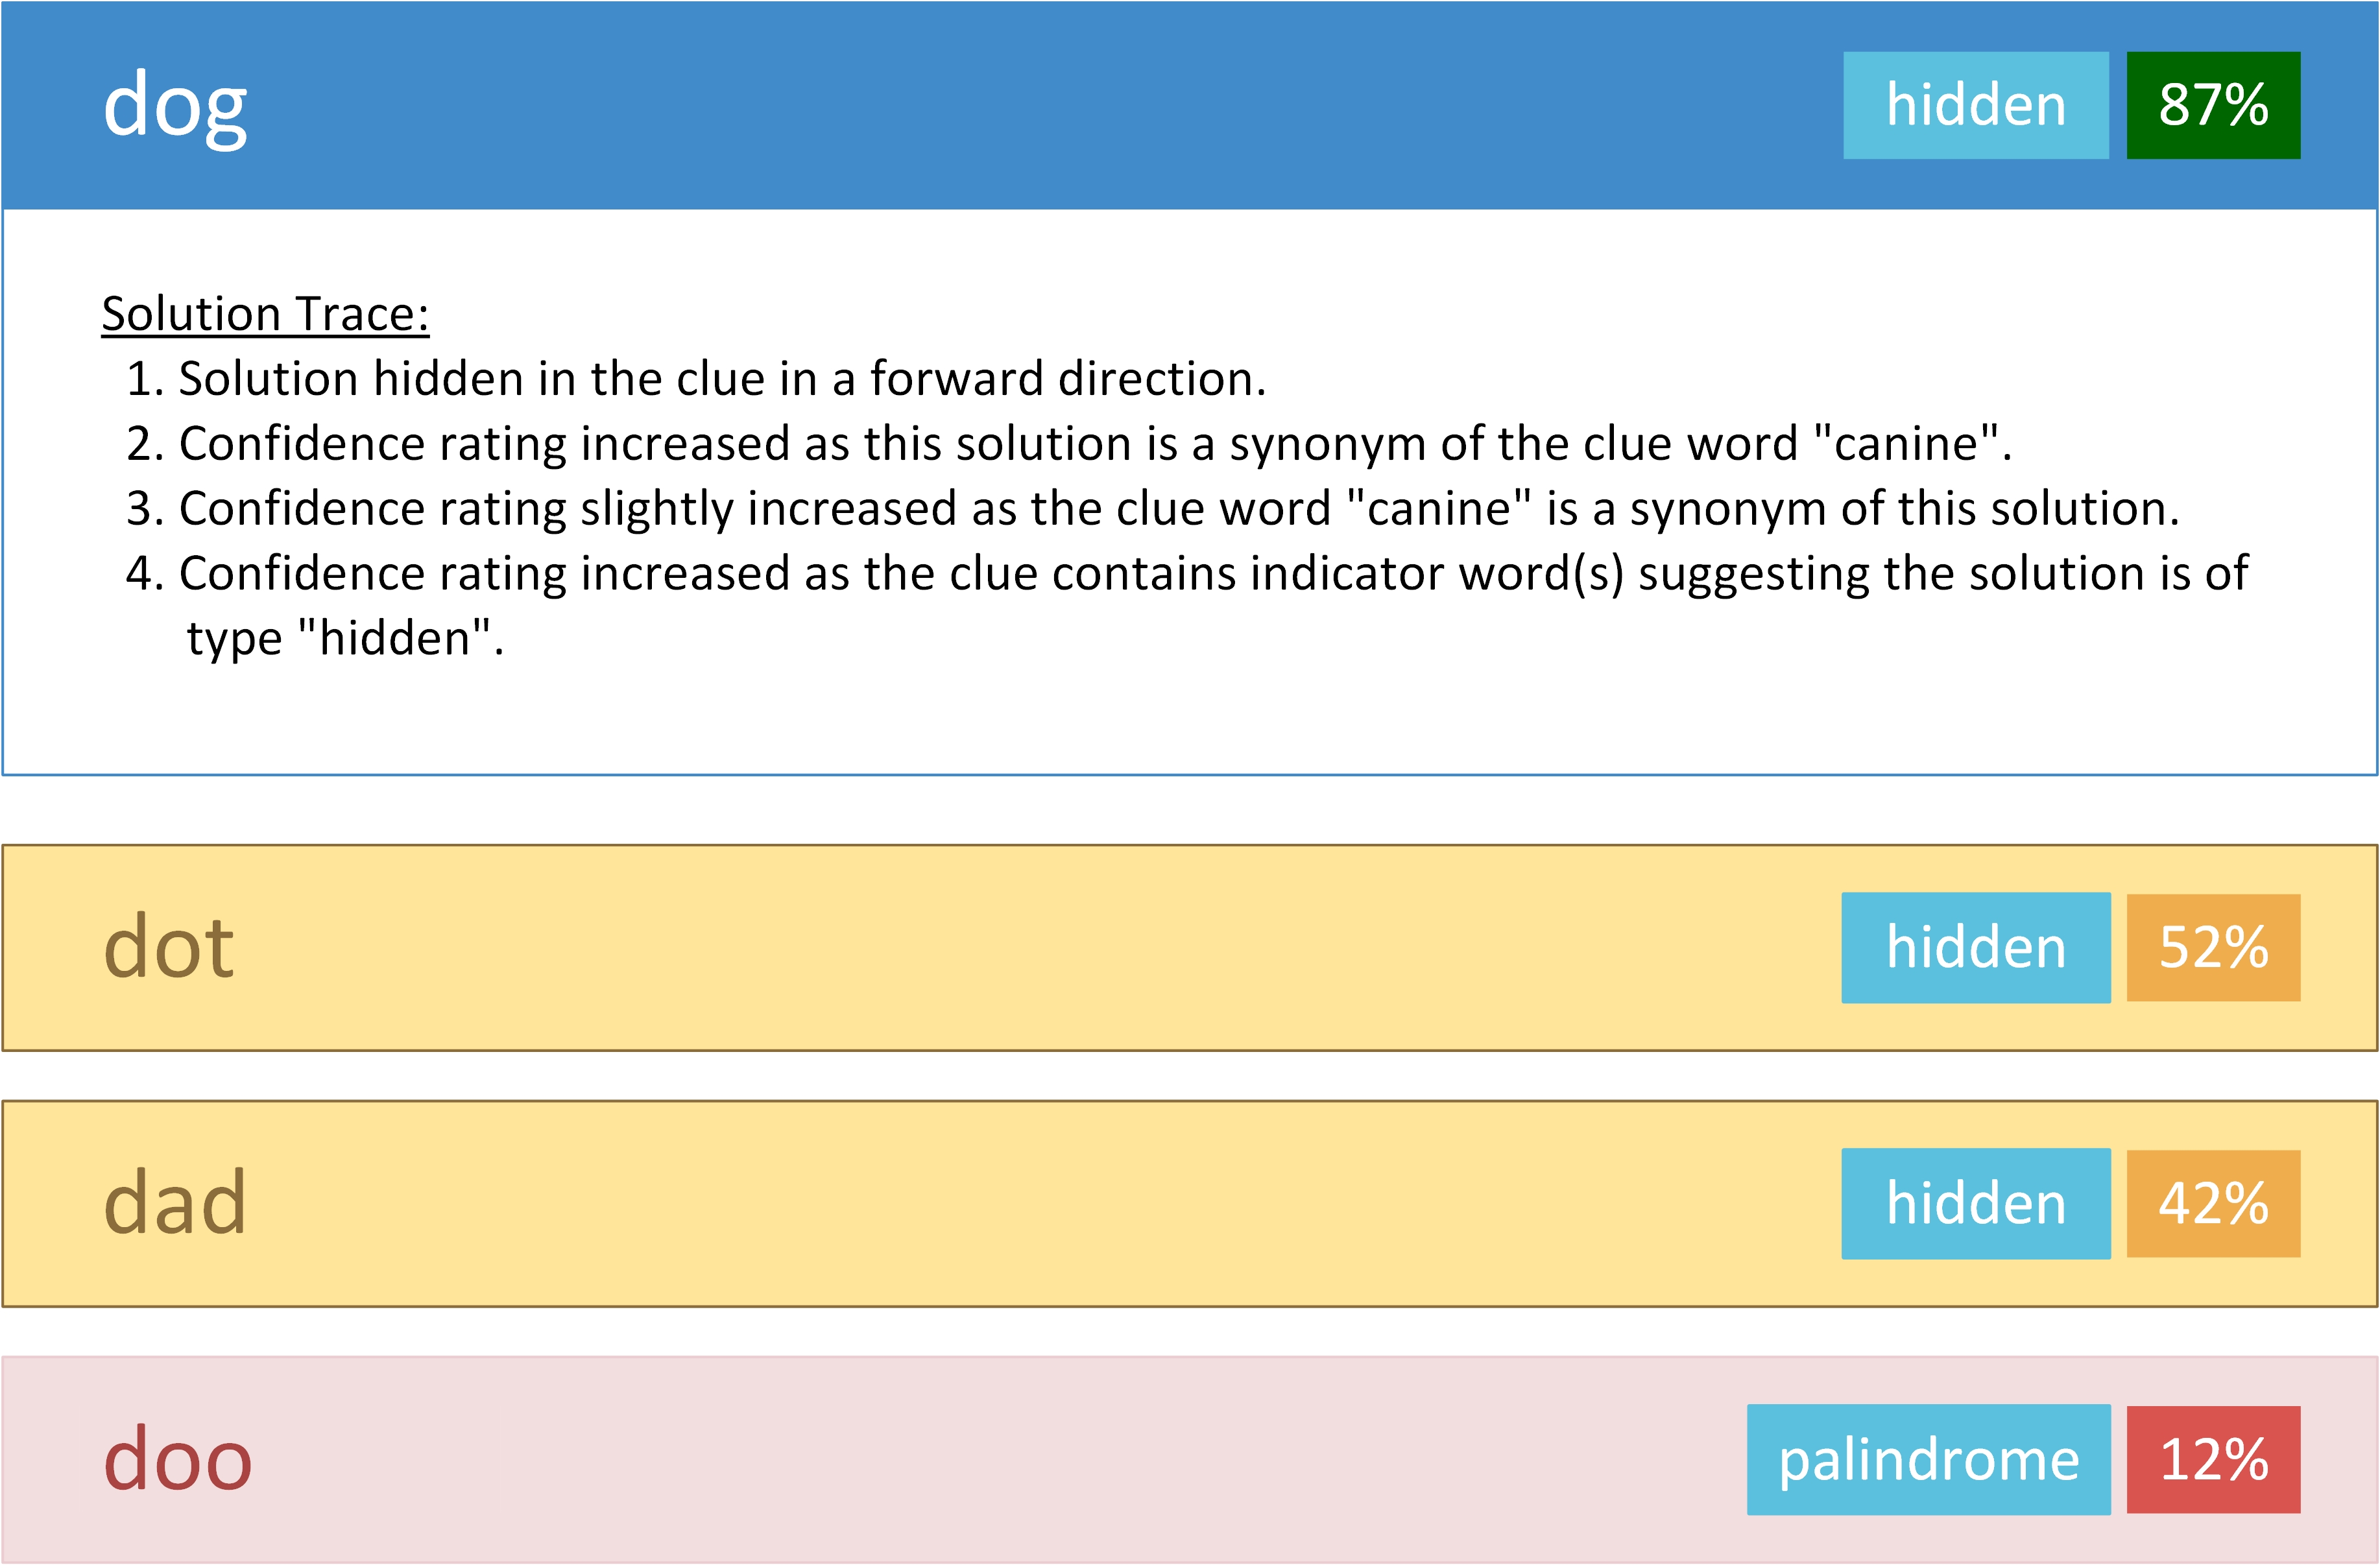
\includegraphics[width=0.8\textwidth]{ui/results_primary.jpg}
  \caption{Results list displaying the top answer in blue}
  \label{fig:results_primary}
\end{figure}

Each of the panels are ``clickable'', meaning that if any given panel is 
selected then the solution trace will be displayed, whilst previously selected 
panels will be `closed' (as shown in Figure \ref{fig:results_secondary}). The 
main reason behind this is to reduce the amount of scrolling a user has to do, 
especially for those without a mouse.

Each solution is awarded a colour based upon the confidence rating. Blue refers 
to a top answer, whilst the remaining colours (green, yellow and red) indicate 
the likely hood of the solution being correct. 

This will allow the end user to immediately deduce that `green' results are 
more likely to be correct in comparison to `red results', and that a `blue' 
result is likely to be correct.

\begin{figure}[H]
  \centering
  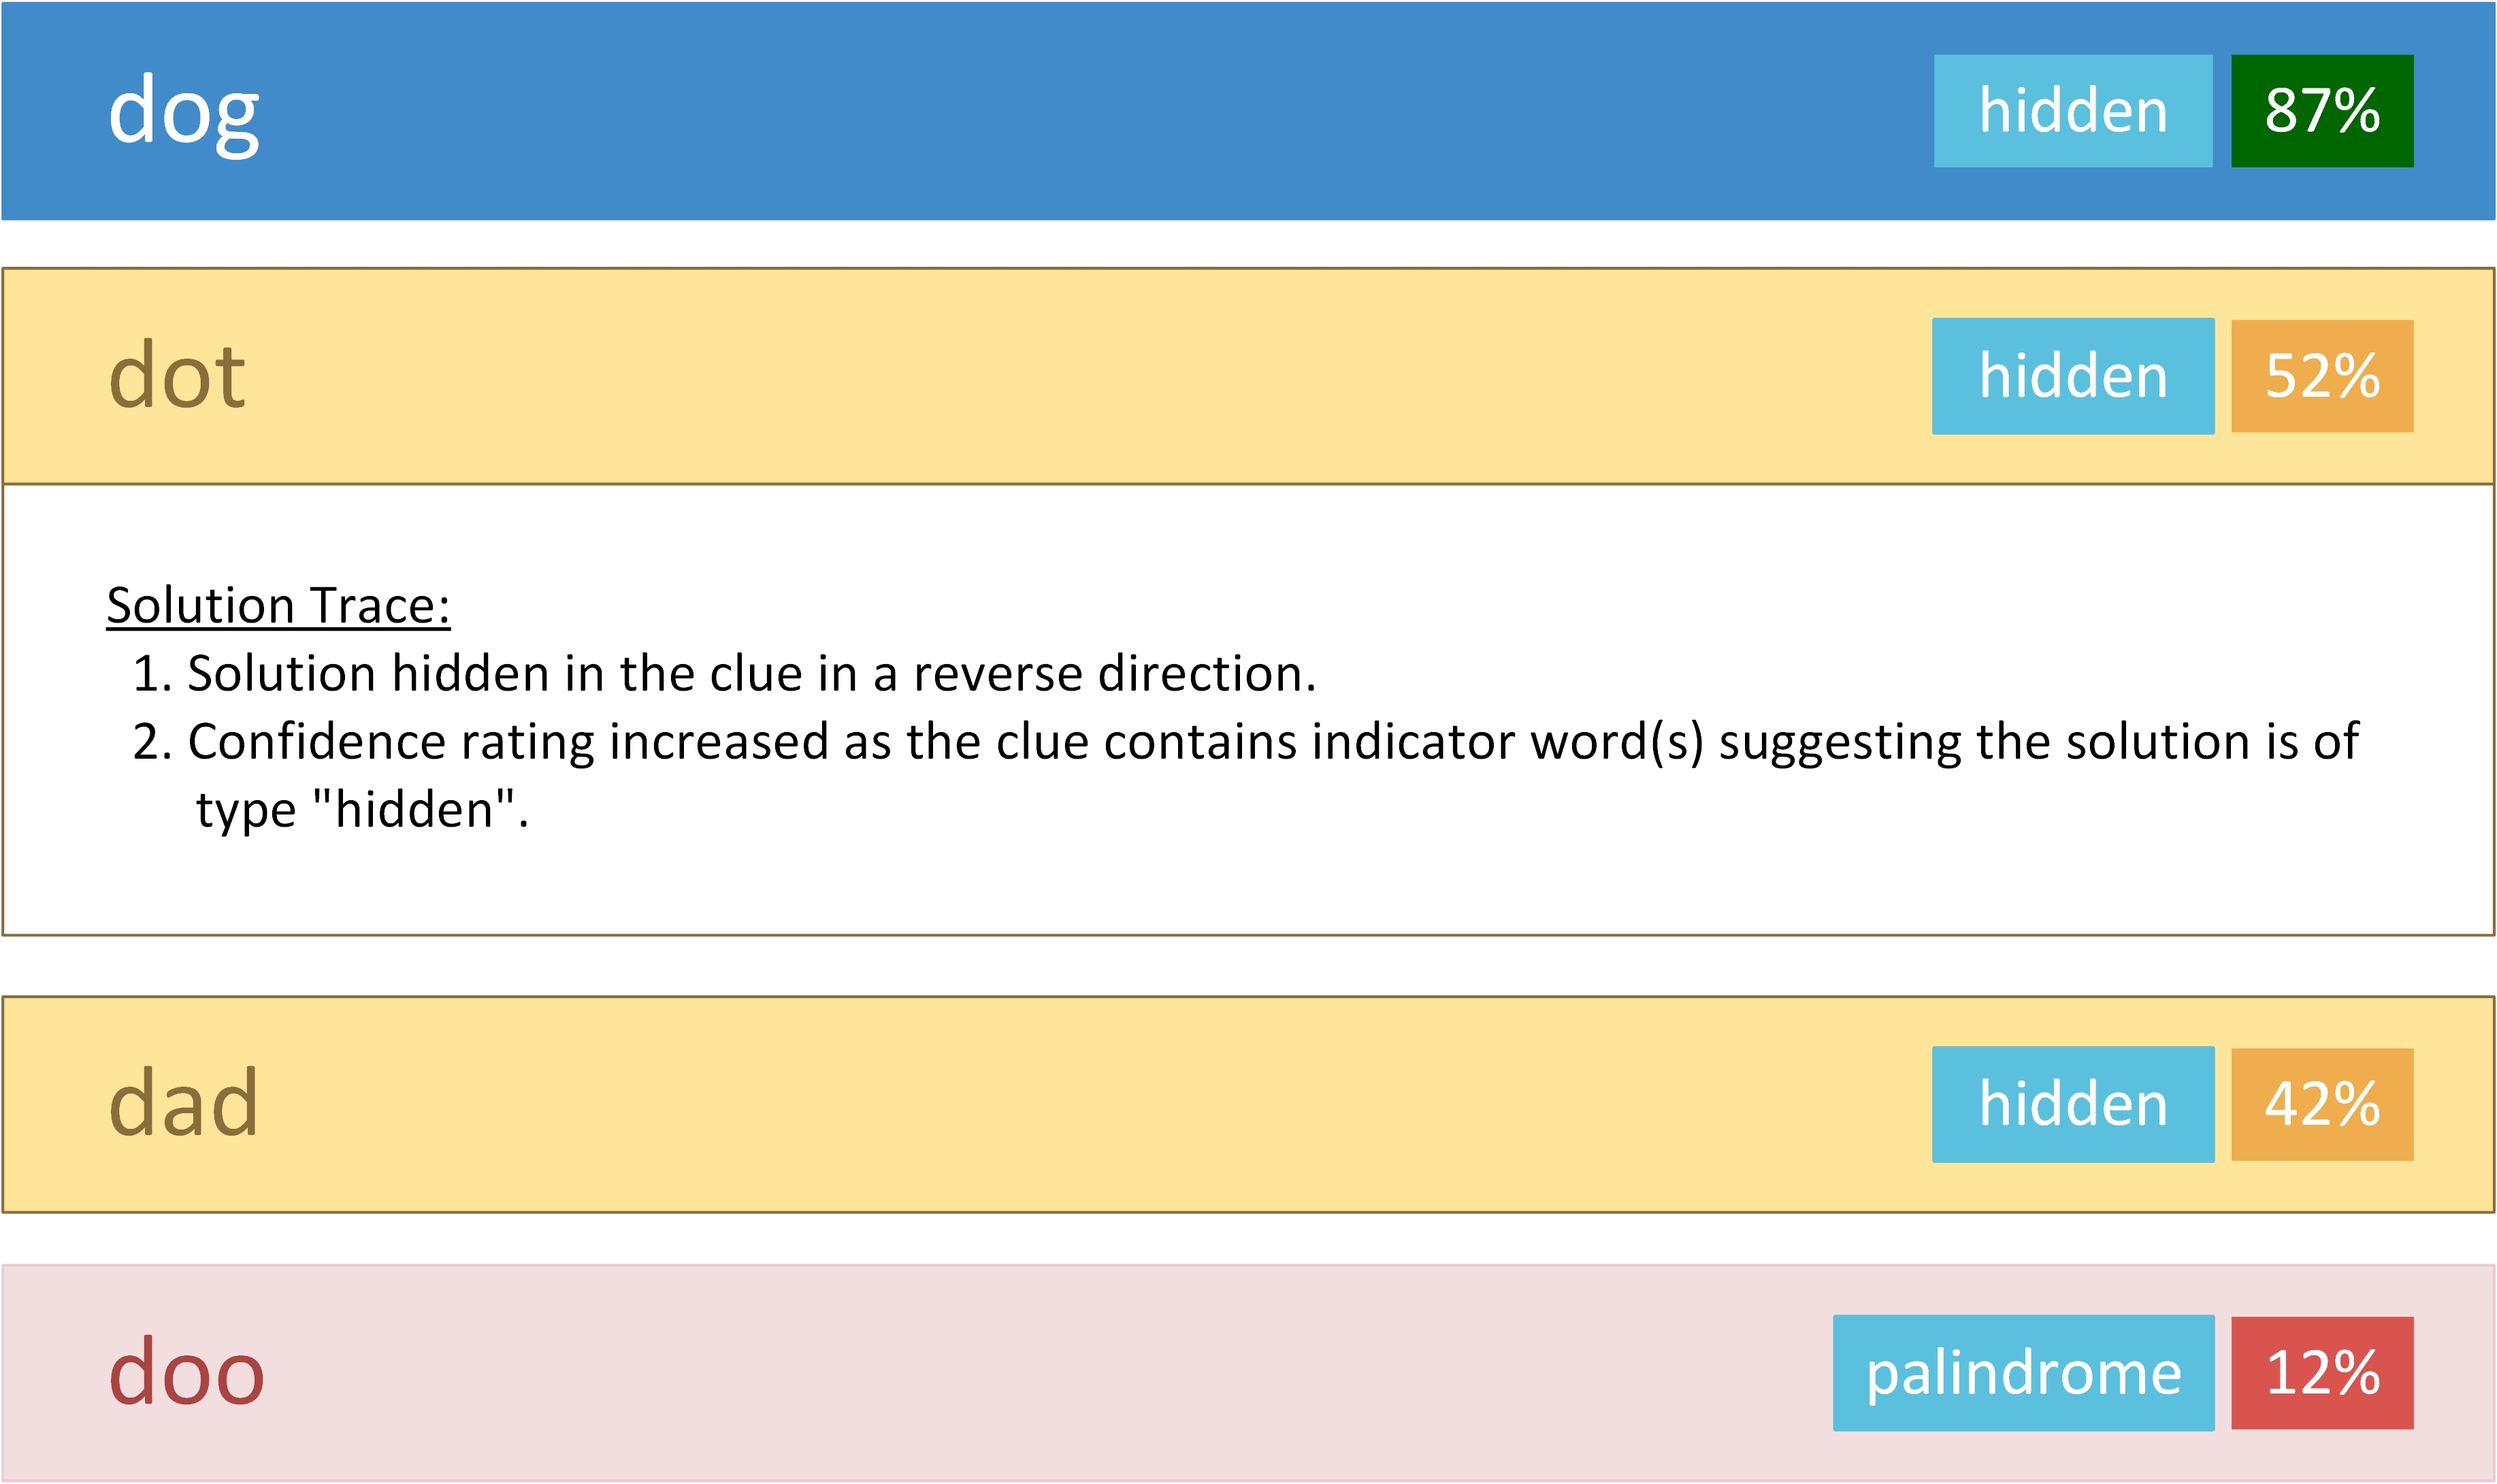
\includegraphics[width=0.8\textwidth]{ui/results_secondary.jpg}
  \caption{Results list displaying alternative solutions}
  \label{fig:results_secondary}
\end{figure}
